\documentclass[ignorenonframetext,hyperref={pdftex,unicode}]{beamer}

\usetheme{AndrejZ}

\title{Свой уласны Dropbox, з календаром, кантактамі і RSS}
\author[Андрэй Захарэвіч]{Андрэй Захарэвіч\\ andrej@zahar.ws}


\begin{document}

\frame{\titlepage} 


\section{Мэты і задачы} 

\begin{frame}{Што мы хацелі атрымаць} 
	Для пачатку хацелася б атрымаць незалежны ад пастаўшчыка інструмент для штодзённых воблачных задач, якія звычайна мы давяраем карпарацыям кшталту Dropbox Inc, Google Inc і іншым. \pauseАсноўныя задачы, якія я б хацеў пакрыць:
	\begin{itemize}
		\item Воблачнае файлавае сховішча/файлаабменнік
		\item Кантакты і календар
		\item RSS
		\item Спасылкі
	\end{itemize}
\end{frame}

\begin{frame}{Файлаабменнік}
	\begin{itemize}
		\item Звычайныя магчымасці па абнаўленню файлаў з адной крыніцы на ўсе месцы, дзе ляжыць яго копія
		\item Магчымасць стварыць агульны набор рэсурсаў для некалькіх карытальнікаў
		\item Магчымасць падзяліцца спасылкай на нейкі файл з кім заўгодна (з нейкім механізмам абмежавання доступа)
		\item Кліент пад Linux для сінхранізацыі ўсяго акаўнта ці асобных яго папак. Пажадана, каб дазваляў дадаваць некалькі акаўнтаў
		\item Кліент пад Android з магчымасцю выбарачнай сінхранізацыі да ўзроўню асобнага файла
	\end{itemize}
\end{frame}

\begin{frame}{Кантакты і календар}
	\begin{itemize}
		\item Цэнтралізаванае сховішча для календара і кантактаў з магчымасцю сінхранізацыі на прылады Android. У ідэале каб сінханізацыя адбывалася гэтак жа, як са звычайнымі правайдэрамі, то бок как не абмяжоўваць спіс праграм, якія потым з гэтымі кантактамі ці календарнымі запісамі змогуць працаваць
		\item Зручны (хаця б мінімальна) інтэрфейс для кампьютэра з магчымасцю аб’ядноўваць кантакты ў групы
		\item Групы кантактаў павінны быць бачныя і даступныя для любых аперацый як з кампа, так і з тэлефона
		\item Магчымасць імпарту кантактаў і календара ў Thunderbird
		\item Магчымасць экспарту у файл і пераносу на іншы сервер
	\end{itemize}
\end{frame}

\begin{frame}{RSS}
	\begin{itemize}
		\item Магчымасць чытаць як з кампьютэра, так і з Android-прылад
		\item Магчымасць дадаваць стужкі з кампьютэра і Андроід-прылад
		\item Магчымасць сінхранізаваць стан (прачытаны, пазначаны як цікавы) для розных працоўных месцаў
		\item У ідэале, магчымасць атрымаць доступ праз вэб-інтэрфейс
		\item Магчымасць экспарту у файл і пераносу на іншы сервер
	\end{itemize}
\end{frame}

\begin{frame}{Спасылкі}
	\begin{itemize}
		\item Магчымасць чытаць як з кампьютэра, так і з Android-прылад
		\item Магчымасць дадаваць з кампьютэра і Андроід-прылад
		\item Групіроўка па групах ці тэгах, даступная для ўсіх кліентаў
		\item Магчымасць экспарту у файл і пераносу на іншы сервер
	\end{itemize}
\end{frame}

\section{Усталёўка і настройкі}
\begin{frame}{Усталёўка: пачатак}
	Магчымыя варыянты устаноўкі неблага апісаныя ў афіцыйным кіраўніцтве [1]. Па-сутнасці ёсць тры асноўных варыянта:
	\begin{itemize}
		\item Узяць зыходнікі і самастойна іх ўжыць на сваім серверы
		\item Узяць пакет пад ваш дыстрыбутыў і паставіць самастойна
		\item Дадаць рэпазітар для вашага дыстрыбутава са сборачнай сістэмы ў вашую сістэму
	\end{itemize}
\end{frame}

\begin{frame}{Усталёўка: базавая канфігурацыя}
	Пасля ўсталёўкі трэба будзе выканаць канфігурацыю, зайшоўшы http://localhost/owncloud [1]
	\begin{itemize}
		\item Пароль і імя карыстальніка для адміністратара
		\item Адрас катагола з дадзенымі
		\item Настройка базы дадзеных [4]
		\item *Давераныя дамены
		\item *Правы доступа на папкі
		\item *Загрузка вялікіх файлаў [5]
	\end{itemize}
\end{frame}

\begin{frame}{Усталёўка: працяг настройкі канфігурацыі}
	Неблага выканаць яшчэ дададковыя крокі для наладкі бяспекі для воблака. Вельмі раю скрарыстацца парадамі з адпаведнага раздзела кіраўніцтва [3]. 

	Хаця, варта прызнаць, не ўсе парады аднолькава карысныя ва ўсіх умовах. Спроба настроіць кэш (пра што нават нагадвае старонка адміністравання) можа прывесці да часовай недаступнасці воблака ці заўважных праблем з хуткасцю працы. А вось абмежаванне логаў часам можа заўважна памяньшаць затрымку паміж запытам і адказам.
\end{frame}

\begin{frame}{Бясплатная тэставая пляцоўка}
	Пазнаёміцца з працай і настройкамі можна на дэма-сайце \url{https://demo.owncloud.org}. Карыстальнік і пароль test. 

	\begin{center}
 		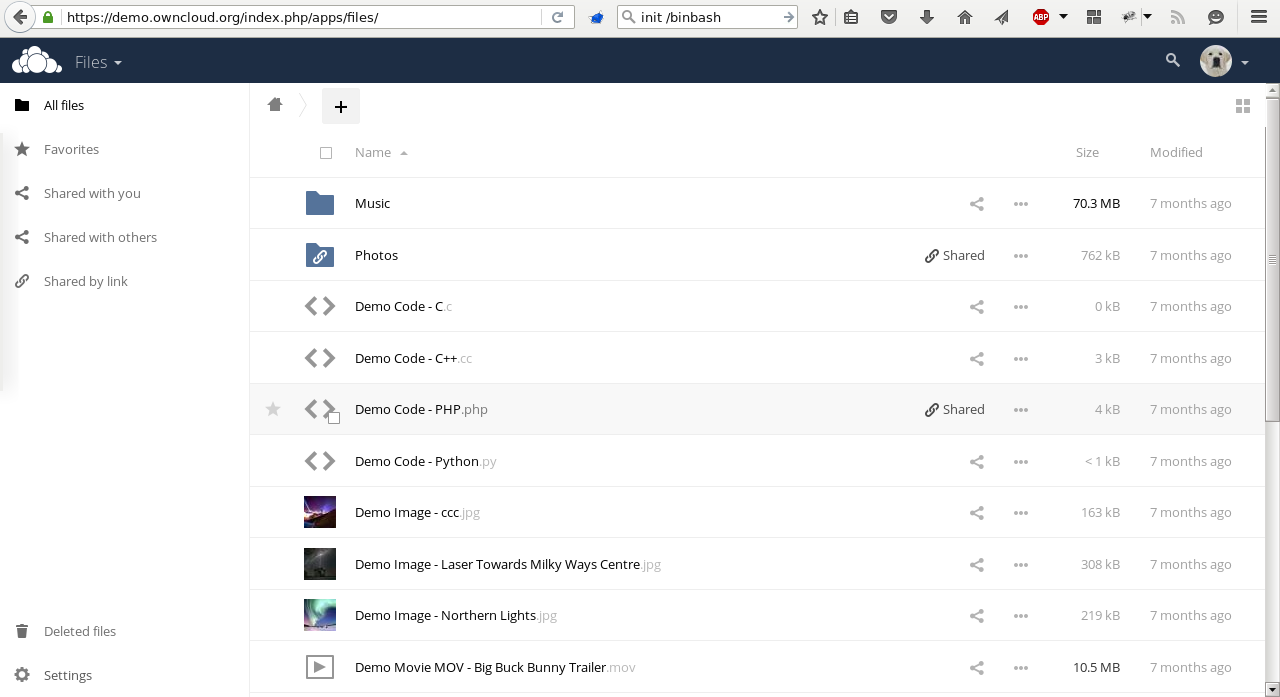
\includegraphics[height=0.5\textheight,keepaspectratio]{demo}
	\end{center}
	
	Выдатная пляцоўка каб без дадатковых выдаткаў паглядзець на базавы функцыянал і асноўныя плугіны. Дарэчы, такім чынам я адпрацоўваў імпарт кантактаў.Хаця, нажаль, набор плагінаў там даволі моцна абмежаваны.
\end{frame}

\begin{frame}{Кіраванне плугінамі}
	Кіраваць наборам актыўных плугінаў можна праз пункт Apps верхняга меню.

	\begin{center}
 		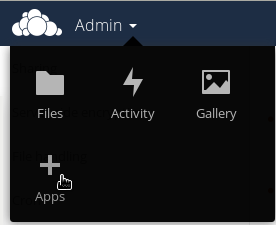
\includegraphics[height=0.4\textheight,keepaspectratio]{apps}
	\end{center}
\end{frame}

\frame{\questionslide}

\begin{frame}[allowframebreaks]{Спіс літаратуры і спасылкі}
	\begin{thebibliography}{10}
	\beamertemplatetextbibitems
	\bibitem{}
		{\sc \href{https://doc.owncloud.org/server/8.2/admin\_manual/installation/index.html}{ownCloud Server Administration Manual: Installation}};
	\bibitem{}
		{\sc \href{https://doc.owncloud.org/server/8.2/admin\_manual/configuration\_server/performance\_tuning.html}{ownCloud Server Administration Manual: Server Tuning \& Performance Tips}};
	\bibitem{}
		{\sc \href{https://doc.owncloud.org/server/8.2/admin\_manual/configuration\_server/harden\_server.html?highlight=security}{ownCloud Server Administration Manual: Hardening and Security Guidance}};
	\bibitem{}
		{\sc \href{https://doc.owncloud.org/server/8.2/admin\_manual/configuration\_database/linux\_database\_configuration.html}{ownCloud Server Administration Manual: Database Configuration}};
	\bibitem{}
		{\sc \href{https://www.ssllabs.com/ssltest/}{Qualys SSL Labs SSL Server Test}};
	\bibitem{}
		{\sc \href{https://doc.owncloud.org/server/8.2/admin\_manual/configuration\_files/big\_file\_upload\_configuration.html}{ownCloud Server Administration Manual: Uploading big files}};
	\bibitem{}
		{\sc \href{https://owncloud.com/products/desktop-clients/}{ownCloud Desktop Clients}};
	\bibitem{}
		{\sc \href{https://play.google.com/store/apps/details?id=com.owncloud.android}{ownCloud client for Android}};
	\bibitem{}
		{\sc \href{http://manandkeyboard.tk/2015/02/26/google-to-owncloud-contacts-and-calendar/}{Man and Keyboard: Google to Owncloud, Contacts and Calendar}};
	\bibitem{}
		{\sc \href{https://play.google.com/store/apps/details?id=tk.drlue.icalimportexport}{iCal Import/Export CalDAV}};
	\bibitem{}
		{\sc \href{http://flailingmonkey.com/moving-contacts-calendar-google/}{Moving your Contacts and Calendar Away from Google}};
	\bibitem{}
		{\sc \href{http://blog.mehl.mx/2014/birthday-calendar-with-owncloud-via-caldav/}{Birthday Calendar with ownCloud via CalDAV}};
	\bibitem{}
		{\sc \href{https://play.google.com/store/apps/details?id=de.luhmer.owncloudnewsreader}{ownCloud News Reader}};
	\bibitem{}
		{\sc \href{https://play.google.com/store/apps/details?id=cz.nethar.owncloudbookmarks}{ownCloud Bookmarks}}.
	\end{thebibliography}
\end{frame}

\begin{frame}{Ужытыя малюнкі}
	\begin{thebibliography}{10}
	\beamertemplatetextbibitems
	\bibitem{}
		{\sc \href{http://amai-biscuit.deviantart.com/art/FreeBSD-Badge-345132138}{FreeBSD Badge}} by {\sc \href{http://amai-biscuit.deviantart.com/}{amai-biscuit}};
	\bibitem{}
		{\sc \href{https://www.flickr.com/photos/nmcmanus/338391435}{Easy Button}} by {\sc \href{https://www.flickr.com/photos/nmcmanus/}{Civilian Scrabble}};
	\bibitem{}
		{\sc \href{https://www.flickr.com/photos/martinaphotography/6428406857}{66/365 Another Creepy One}} by {\sc \href{https://www.flickr.com/photos/martinaphotography/}{martinak15}};
	\bibitem{F-16}
		{\sc \href{https://commons.wikimedia.org/wiki/File:F-15\_takeoff.jpg}{F-15\_takeoff}} by {\sc USAF};
	\bibitem{}
		{\sc \href{https://www.flickr.com/photos/toasty/914441359}{Bang!}} by {\sc \href{https://www.flickr.com/photos/toasty/}{Kenneth Lu}}.
	\end{thebibliography}
\end{frame}

\end{document}
